\documentclass[margin=1mm]{standalone}
\usepackage{graphicx}
\usepackage{amsmath,amssymb,bbm,amsfonts,amsopn}
\usepackage{stackrel,floatrow,url,lipsum,hyperref,mathrsfs,pgf,tikz,pgfplots,tikz-cd}
\usepackage{colortbl,stackengine,euscript,mathtools,subcaption,pbox,xspace,verbatim}
\usepackage{tikz}

\usepackage{xcolor}
\definecolor{peach}{HTML}{ecbcb2}
\definecolor{azure}{HTML}{57caff}

\tikzset{every node/.style={font=\small}}

\begin{document}
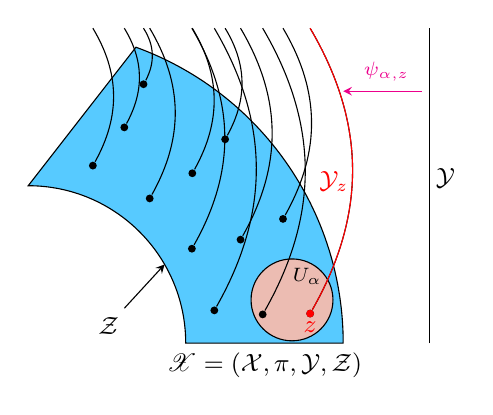
\begin{tikzpicture}[>=stealth]
\draw[fill=azure](2,0)--(4,0)node[midway,below]{$\mathscr{X} = \left( \mathcal{X}, \pi, \mathcal{Y}, \mathcal{Z} \right)$}arc(0:70:4)--(90:2)arc(90:0:2)--cycle;

\draw[fill=peach] (3.35,0.55) circle (0.52cm)node[left,xshift=5mm,yshift=3mm]{\scriptsize{$U_\alpha$}};

\draw[fill=red](5.1,0)--(5.1,4)node[near end,xshift=2mm,yshift=-9mm]{$\mathcal{Y}$};
\draw[->] (20:1.3)node[below,xshift=-2mm]{$\mathcal{Z}$}--(30:2);

\begin{scope}[bend right]
\foreach \i[count=\x] in {10,30,50,70}
{\node(a\x)[circle,fill,inner sep=1pt]at (\i:2.4){};
\draw(a\x)to(a\x|-0,4);}

\foreach \i[count=\x] in {7,26,46,66}
{\node(b\x)[circle,fill,inner sep=1pt]at (\i:3){};
\draw(b\x)to(b\x|-0,4);}

\foreach \i[count=\x] in {6,26,46,66}
{\node(c\x)[circle,fill,inner sep=1pt]at (\i:3.6){};
\draw(c\x)to(c\x|-0,4);}

\foreach \i[count=\x] in {6}
{\node[fill=red](c\x)[circle,fill,inner sep=1pt]at (\i:3.6){};
\draw[red](c\x)to(c\x|-0,4)node[below,xshift=0mm,yshift=-36mm]{$z$}node[below,xshift=3mm,yshift=-17mm]{$\mathcal Y_z$};}

\path(c1)to coordinate[near start](d)(c1|-0,4);
\end{scope}

\draw[magenta][<-](4,3.2) -- (5,3.2)node[near end,above,xshift=-2mm]{\scriptsize{$\psi_{\alpha,z}$}};

% \draw[purple][<-](d)--+(0.3,-0.2)node[right]{$\color{red}{\mathcal{Y_{\mathbf{z}}}}$};

\end{tikzpicture}
\end{document}
